% HackerSignal — NeurIPS 2026 Evaluations & Datasets Track
% Submission version (anonymous, double-blind)
%
% To compile:
%   pdflatex HackerSignal_neurips2026.tex
%   bibtex   HackerSignal_neurips2026
%   pdflatex HackerSignal_neurips2026.tex
%   pdflatex HackerSignal_neurips2026.tex
%
% Track options:
%   Submission (anonymous):   \usepackage[eandd]{neurips_2026}
%   Camera-ready:             \usepackage[eandd, final]{neurips_2026}
%   Preprint (arXiv):         \usepackage[preprint]{neurips_2026}

\documentclass{article}

\usepackage[eandd]{neurips_2026}  % Evaluations & Datasets Track

\usepackage[utf8]{inputenc}
\usepackage[T1]{fontenc}
\usepackage{hyperref}
\usepackage{url}
\usepackage{booktabs}
\usepackage{amsfonts}
\usepackage{amsmath}
\usepackage{nicefrac}
\usepackage{microtype}
\usepackage{xcolor}
\usepackage{graphicx}
\usepackage{multirow}
\usepackage{array}
\usepackage{subcaption}
\usepackage{pifont}
\usepackage{wrapfig}

\newcommand{\etg}{\textsc{HackerSignal}}
\newcommand{\todo}[1]{\textcolor{red}{[\textbf{TODO:} #1]}}
\newcommand{\cmark}{\ding{51}}
\newcommand{\xmark}{\ding{55}}

\title{\etg: A Large-Scale Multi-Source Dataset Linking Hacker Community
       Discourse to the CVE Vulnerability Lifecycle}

\author{%
  Anonymous Author(s) \\
  Affiliation \\
  \texttt{email@domain.com}
}

\begin{document}

\maketitle

\begin{abstract}

We introduce HackerSignal, a benchmark for temporal out-of-distribution cyber threat intelligence (CTI) and cross-source CVE linkage. HackerSignal aggregates \textbf{7.45 million exact-deduplicated documents} from \textbf{64 public forum/source identifiers} spanning eight source layers and a 36-year window (1990--2026). In contrast to other publicly accessible cybersecurity datasets, HackerSignal is among the first public benchmark datasets that maps the full potential exploit to vulnerability trajectory from hacker community discourse, exploit databases with working and proof of concept exploits, vulnerability advisories, and software fix commits. HackerSignal creates these linkages through a shared CVE identifier space while preserving source-specific release modes to support a range of unique Artificial Intelligence (AI)-enabled cybersecurity analytics tasks. In this paper, we summarize HackerSignal and illustrate three selected benchmark tasks it uniquely supports: (1)~\emph{CVE linkage retrieval} (cross-source temporal out-of-distribution entity grounding); (2)~\emph{exploit type classification} (8-class vulnerability type prediction with temporal OOD evaluation); and (3)~\emph{temporal generalization} (prospective CVE-disjoint evaluation where $C_{\text{train}} \cap C_{\text{test}} = \emptyset$). All tasks use temporal splits to evaluate prospective generalization. We release source-shortcut and leakage diagnostics; manual-audit packets; a datasheet; and a release-governance addendum to support the dissemination of the dataset. HackerSignal's code, data, and Croissant metadata are available at \href{https://huggingface.co/datasets/DatasetSubmission/HackerSignal}{\texttt{hf.co/datasets/DatasetSubmission/HackerSignal}} (data) and \href{https://anonymous.4open.science/r/hackersignal-8A2F/}{\texttt{anonymous.4open.science/r/hackersignal-8A2F}} (code).
\end{abstract}

\section{Introduction}

Understanding how cyber threats emerge, propagate, and relate to vulnerabilities is a central challenge in modern applied cybersecurity. Signals that tracks this trajectory is distributed across heterogeneous text-based sources, including: (1) hacker forums where exploits are first discussed, (2) public exploit databases where proof-of-concept code is released, (3) official vulnerability advisories such as the National Vulnerability Database, CISA's Known Exploited Vulnerabilities, and GitHub Advisory where threats are cataloged, and (4) open-source repositories where fixes are committed. Extant public datasets in this domain often span a single or subset of these layers~\citep{crimebb2018} and are usually not publicly released~\citep{ampel2020dtl}. A survey of CTI extraction from text identifies advisory records and threat reports as the dominant labeled sources studied, with exploit-archive and PoC-focused benchmarks remaining scarce~\citep{rahman2023cti}; a companion survey of cybercrime community research corroborates that structured datasets linking forum posts to formal vulnerability records are largely absent from the public literature~\citep{hughes2024cybercrime}. HackerSignal addresses this gap with a temporally structured, multi-source corpus and benchmark spanning the full advisory-to-exploit trajectory, enabling downstream CTI analytics tasks. HackerSignal makes three key contributions:

\begin{enumerate}
  \item \textbf{A temporally grounded CTI corpus} of 7.45M documents from 64 public forum/source identifiers across eight source layers (hacker communities, exploit archives, vulnerability references, exploit Q\&A references, advisories, bug-bounty disclosures, fix commits, and exploitation references), with CVE linkage metadata connecting vulnerability identifiers to the texts that discuss them. The 6.97M-row hacker community subcorpus alone (spanning 56 forums across darkweb marketplaces, security discussion boards, and multilingual hacker communities) supports diverse NLP tasks beyond our three benchmarks, including exploit code summarization, security content classification, topic modeling, community interaction analysis, and cross-lingual CTI extraction.

  \item \textbf{Three benchmark tasks} with temporal train/val/test splits that test progressively harder generalization in (1) cross-source CVE linkage retrieval, (2) 8-class exploit type classification, and (3) CVE-disjoint temporal generalization ($C_{\text{train}} \cap C_{\text{test}} = \emptyset$), accompanied by shortcut/leakage diagnostics.

  \item \textbf{A full model ladder and governance artifacts} from BM25 through four dense bi-encoders (MiniLM, mpnet, BGE, E5), bag-of-words classifiers (Decision Tree, TF-IDF+LR, SVM), recurrent neural networks (RNN, GRU, LSTM, BiLSTM), a domain-specific transformer (SecBERT), and hybrid sparse+dense retrieval, alongside source-shortcut diagnostics, manual-audit packets, and a release-governance addendum.
\end{enumerate}

\noindent Figure~\ref{fig:pipeline} provides an overview of the complete pipeline of the proposed dataset, including eight source layers unified through a shared CVE identifier space, then channeled into three benchmark tasks with temporal controls. Temporal splits are necessary in our context as real CTI systems must generalize to threats that did not exist at training time~\citep{koh2021wilds}. We explicitly audit the dataset for temporal and source leakage~\citep{kapoor2023leakage} because benchmark claims are otherwise easy to inflate (discussed in Section 3.

\section{Related Work}

\paragraph{Hacker-community cyber threat intelligence.} Early hacker-forum CTI work treated underground communities as a source of proactive intelligence about tools, actors, and emerging attack capabilities~\citep{samtani2015assets, samtani2017jmis}. The AZSecure Hacker Assets Portal operationalized this as a situational awareness platform~\citep{samtani2021hap}, while parallel work modeled threat emergence over time via diachronic graph embeddings~\citep{samtani2020dgef} and mobile malware identification~\citep{grisham2017mobile}. The resulting artifacts are operational systems rather than reusable ML benchmarks, since their data remains proprietary. \citet{rahman2023cti} survey automated CTI extraction from text, observing that collections often concentrate on the advisory and threat-report tier, while exploit-archive and PoC-focused benchmarks remain scarce. \citet{hughes2024cybercrime} systematize research on the cybercrime community and demonstrate a persistent shortage of ground-truth datasets. Most publicly collected forum data lacks structured labels linking posts to formal vulnerability records.

\paragraph{Exploit labeling and vulnerability linkage.}
The closest predecessor to HackerSignal is in the field of exploit labeling research. Prior methods labeled hacker-forum exploit source code via deep transfer learning from professional exploit repositories~\citep{ampel2020dtl} and later extended this with pre-initialization, multi-layer transfer, and self-attention~\citep{ampel2024misq}. For cross-source linkage, an attention-based deep-structured semantic model linked dark-web exploits to known vulnerabilities, yielding 52,590 linkages~\citep{samtani2022eva}. HackerSignal differs by releasing a governed, temporally split public benchmark that exposes source provenance, weak-label caveats, and a quality-controlled CVE-linkage retrieval task. Finally, the hacker forum collection of~\citet{otto2021isi} aggregates 259K posts from three English-language security communities (AntiOnline, Go4Expert, CipherSpace) and studies exploit-sharing behavior via graph embeddings.

\paragraph{Underground community datasets.} Research has also focused on the general crawling of hacker communities, like a credentialized dataset of darkweb cybercrime forum posts widely used for crime and exploit prediction~\citep{crimebb2018} \citet{nunes2016darknet} presented an operational darknet/deepnet mining system over hacker forums and markets for proactive CTI.The Gayanku~\citep{gayanku2020} dataset provides 3.8M posts from seven darknet marketplaces (Silk Road, Agora, Evolution, et al.) on Kaggle.

\paragraph{Exploit and vulnerability databases.} ExploitDB~\citep{exploitdb} is the salient public exploit archive (50K+ entries, many with CVE IDs). The CVEfixes dataset~\citep{cvefixes2021} links CVEs to fix commits in open-source repositories. NVD~\citep{nvd}, CISA KEV~\citep{cisakev}, and GitHub Advisory~\citep{githubadvisory} are official advisory sources. HackerSignal normalizes all five into a common JSONL schema with CVE keys.

\paragraph{Multilingual CTI.} More general hacker-forum text classification work compared SVM and CNN models for extracting CTI from forum posts~\citep{deliu2017cti}, while \citet{ebrahimi2020crosslingual} showed that non-English hacker forums require cross-lingual approaches that avoid brittle machine translation. CVE severity prediction~\citep{severitypred2017}, exploit labeling~\citep{ampel2024misq}, and exploit-vulnerability linkage~\citep{samtani2022eva} all motivate our task design; HackerSignal operationalizes them as public, temporally split benchmarks.

\paragraph{Benchmark design and evaluation methodology.} BEIR~\citep{thakur2021beir} established that retrieval benchmarks require heterogeneous baseline ladders rather than single-model comparisons. KILT~\citep{petroni2021kilt} showed that knowledge-intensive linking tasks should reward both task success and provenance quality. WILDS~\citep{koh2021wilds} formalized natural arising distribution shifts (including temporal shifts) as first-class benchmark objects, while WRENCH~\citep{zhang2021wrench} demonstrated that weak-supervision evaluation is sensitive to hidden protocol choices, requiring explicit reporting of label sources and aggregation rules. \citet{kapoor2023leakage} documented widespread data leakage in ML-for-science benchmarks and proposed structured reporting to make integrity checks legible. Our temporal splits, source-shortcut diagnostics, and audit artifacts are directly informed by these methodological precedents.

\section{Dataset}
\label{sec:dataset}

\subsection{Source Layers}

HackerSignal integrates public hacker-community discourse with sources of exploit, advisory, vulnerability-reference, bug-bounty, and commit-fix in eight source layers (Figure~\ref{fig:pipeline}, left). Table~\ref{tab:corpus-stats} reports the composition of the audited release; Table~\ref{tab:quality-audit} reports quality diagnostics.

\begin{table}[t]
\vspace{-4pt}
\centering
\small
\setlength{\tabcolsep}{4pt}
\caption{Corpus quality diagnostics.}
\label{tab:quality-audit}
\begin{tabular}{lrr}
\toprule
\textbf{Diagnostic} & \textbf{Rows} & \textbf{Share} \\
\midrule
Parseable timestamps        & 7,447,646 & 100.0\% \\
CTI-keyword nonzero         & 1,748,049 &  23.5\% \\
CVE string present          &   360,004 &   4.8\% \\
Short rows ($<$8 tok)       & 1,569,263 &  21.1\% \\
Long rows ($>$3000 tok)     &       815 &  $<$0.1\% \\
Est.\ near-duplicates       &   609,029 &   8.2\% \\
\bottomrule
\end{tabular}
\vspace{-4pt}
\end{table}

\begin{table}[t]
\centering
\small
\setlength{\tabcolsep}{3pt}
\caption{Dataset statistics after exact deduplication. The hacker community layer is expanded by a forum. The remaining layers are single-source. Avg.\ Len = mean whitespace tokens; CVE\% = rows containing an explicit CVE identifier.}
\label{tab:corpus-stats}
\begin{tabular}{llrrrl}
\toprule
\textbf{Source Layer} & \textbf{Source / Forum} & \textbf{\#Docs} & \textbf{Avg Len} & \textbf{CVE\%} & \textbf{Span} \\
\midrule
\multirow{9}{*}{\rotatebox[origin=c]{90}{\footnotesize Hacker Community}}
 & gayanku\_darkweb     & 3,107,038 & 72.6 & $<$0.1 & 2011--17 \\
 & antichat             & 1,819,730 & 39.7 & $<$0.1 & 2002--26 \\
 & evolution\_darkweb   &   471,115 & 65.4 & $<$0.1 & 2014--15 \\
 & antionline           &   462,510 & 73.6 & $<$0.1 & 2001--26 \\
 & persiantools         &   280,293 & 82.1 & $<$0.1 & 2026 \\
 & wwhclub              &   161,026 & 51.3 & $<$0.1 & 2026 \\
 & hackforums           &   151,072 & 31.6 & $<$0.1 & 2009--15 \\
 & go4expert            &   110,345 & 75.1 & $<$0.1 & 2004--26 \\
 & \textit{Other (48 forums)} &   402,885 & 56.5 & 0.1 & 2000--26 \\
\cmidrule{2-6}
 & \textbf{Subtotal}    & \textbf{6,966,014} & \textbf{61.7} & \textbf{$<$0.1} & \textbf{2001--26} \\
\midrule
\multicolumn{2}{l}{Vulnerability Ref (NVD)} &   340,536 & 47.2 & 100.0 & 2002--26 \\
\multicolumn{2}{l}{Exploit Archive}         &    46,653 & 240.0 & 10.5 & 1991--26 \\
\multicolumn{2}{l}{Exploit Q\&A Ref}        &    46,505 & 25.2 & $<$0.1 & 2000 \\
\multicolumn{2}{l}{Advisory Ref}            &    28,684 & 110.8 & 5.0 & 2017--26 \\
\multicolumn{2}{l}{Bug-Bounty Disclosure}   &     9,453 & 191.1 & 6.5 & 2013--24 \\
\multicolumn{2}{l}{Fix-Commit Ref}          &     8,293 & 92.0 & 100.0 & 1999--22 \\
\multicolumn{2}{l}{Exploitation Ref (KEV)}  &     1,508 & 54.4 & 3.8 & 2021--26 \\
\midrule
\multicolumn{2}{l}{\textbf{Total (64 sources)}} & \textbf{7,447,646} & \textbf{62.0} & \textbf{4.8} & \textbf{1991--26} \\
\bottomrule
\end{tabular}
\end{table}

\paragraph{Hacker and security communities (6.97M rows).}
The hacker-community layer captures organic security discourse. This includes, but is not limited to, discussions of exploits, tool sharing, vulnerability commentary, marketplace posts, and peer support across communities. Our collection combines historical forum datasets (e.g., Gayanku, Evolution, and HackForums) with newer publicly accessible sources such as DeepDarkCTI communities, 0x00sec, HackerSploit, and ParrotSec. The largest forums after deduplication are \texttt{gayanku\_darkweb} (3.11M rows), \texttt{antichat} (1.82M), \texttt{evolution\_darkweb} (471K), \texttt{antionline} (463K), \texttt{persiantools} (280K), \texttt{wwhclub} (161K), and \texttt{hackforums} (151K). Forum sources often carry sparse direct CVE mentions and exhibit heterogeneous vocabulary overlap across communities (Figure~\ref{fig:domain-overlap}). These characteristics make CVE linkage from community discourse a nontrivial retrieval problem.

\begin{figure}[t]
\centering
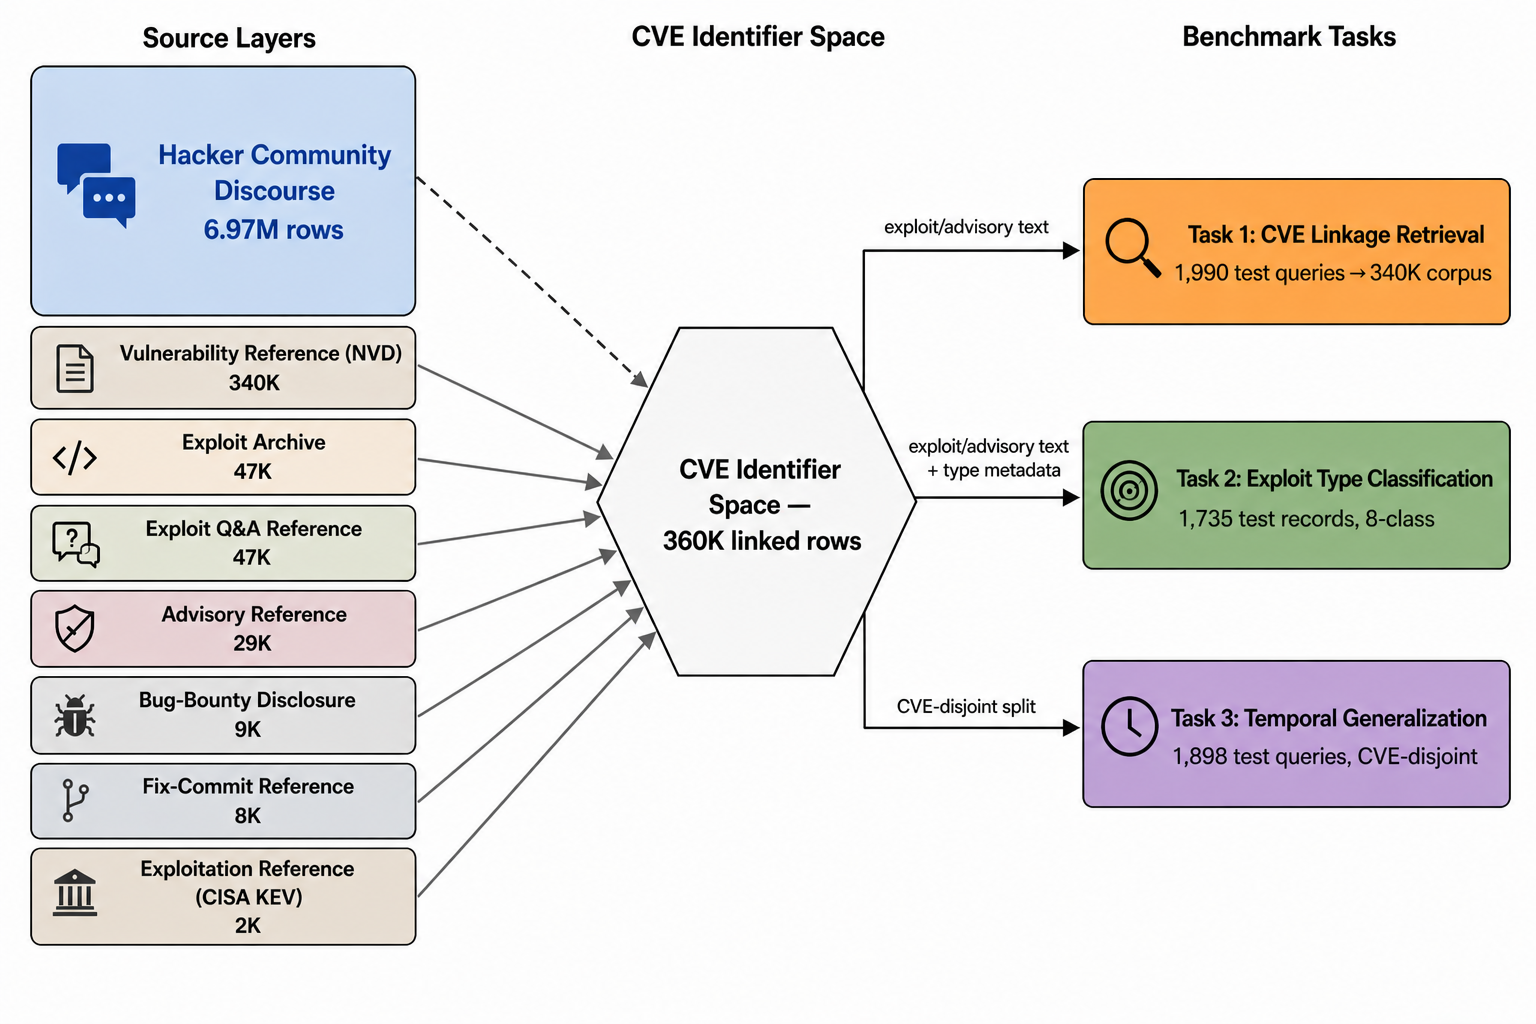
\includegraphics[width=0.8\linewidth]{figures/pipeline_overview.png}
\caption{HackerSignal pipeline overview. Dashed arrows indicate sparse, indirect CVE mentions. Solid arrows indicate direct CVE metadata linkage.}
\label{fig:pipeline}
\end{figure}

\vspace{-0.5 cm}

\paragraph{Reference and supervision layers (482K rows).}
The remaining layers provide CVE-grounded supervision and comparison corpora. NVD CVE descriptions (340,536 rows) form the retrieval corpus for all three benchmark tasks. ExploitDB, 0day.today, Packet Storm, ZeroScience, and Vulnerability-Lab contribute exploit and advisory text. GitHub Advisory, CISA KEV, HackerOne, and CVEfixes contribute structured records for vulnerabilities, bug bounties, known-exploited issues, and fix commits. These sources are separated by \texttt{source\_layer}; thus, experiments can evaluate either community-only discourse or community-plus-context settings.

\subsection{CVE Identifier Space}

All sources are unified through a common JSONL record format and a shared CVE identifier namespace (Figure~\ref{fig:pipeline}, center). Each record carries a SHA-256-derived release identifier, source provenance (\texttt{source\_layer}, \texttt{forum\_id}), cleaned UTF-8 text, an ISO~8601 timestamp, and a pseudonymized author hash. A separate CVE index maps each record to its CVE reference(s) via a foreign key, enabling cross-source joins through the shared identifier space. Of the 7.45M documents, 360,004 rows (4.83\%) contain explicit CVE references, forming the linkage substrate for all three benchmark tasks. The full schema specification is provided in the accompanying datasheet~\citep{gebru2021datasheet}.

\subsection{Collection and Preprocessing}

Data was collected between January and April 2026 via (i)~official APIs (NVD, GitHub Advisory, CISA KEV, HackerOne HuggingFace Hub), (ii)~ingestion of existing public datasets (e.g., Gayanku, HackForums, CVEfixes, DeepDarkCTI, CrackingArena), and (iii)~ethical web scraping of publicly indexed sites (e.g., ExploitDB, Vulnerability-Lab, ZeroScience, 0x00sec, HackerSploit, ParrotSec, Hack The Box, Go4Expert, Full Disclosure). All collection code is released alongside the dataset.

We took four steps to prepare the data for our three proposed tasks. First, we perform text cleaning by normalizing Unicode, stripping HTML tags, replacing URLs, and collapsing extra whitespace. Second, we filtered out low-quality content, including non-English language and posts shorter than 20 characters. Third, we run exact deduplication via SHA-256 hashing and near-deduplication via MinHash-LSH with 128 permutations, 3-character k-shingles, and Jaccard similarities between posts over 0.7. Finally, we divided the posts into temporal train, validation, and test splits. The release removes 814,922 posts. We show the final dataset distribution in Figure~\ref{fig:temporal-heatmap}. 

\begin{figure}[t]
\centering
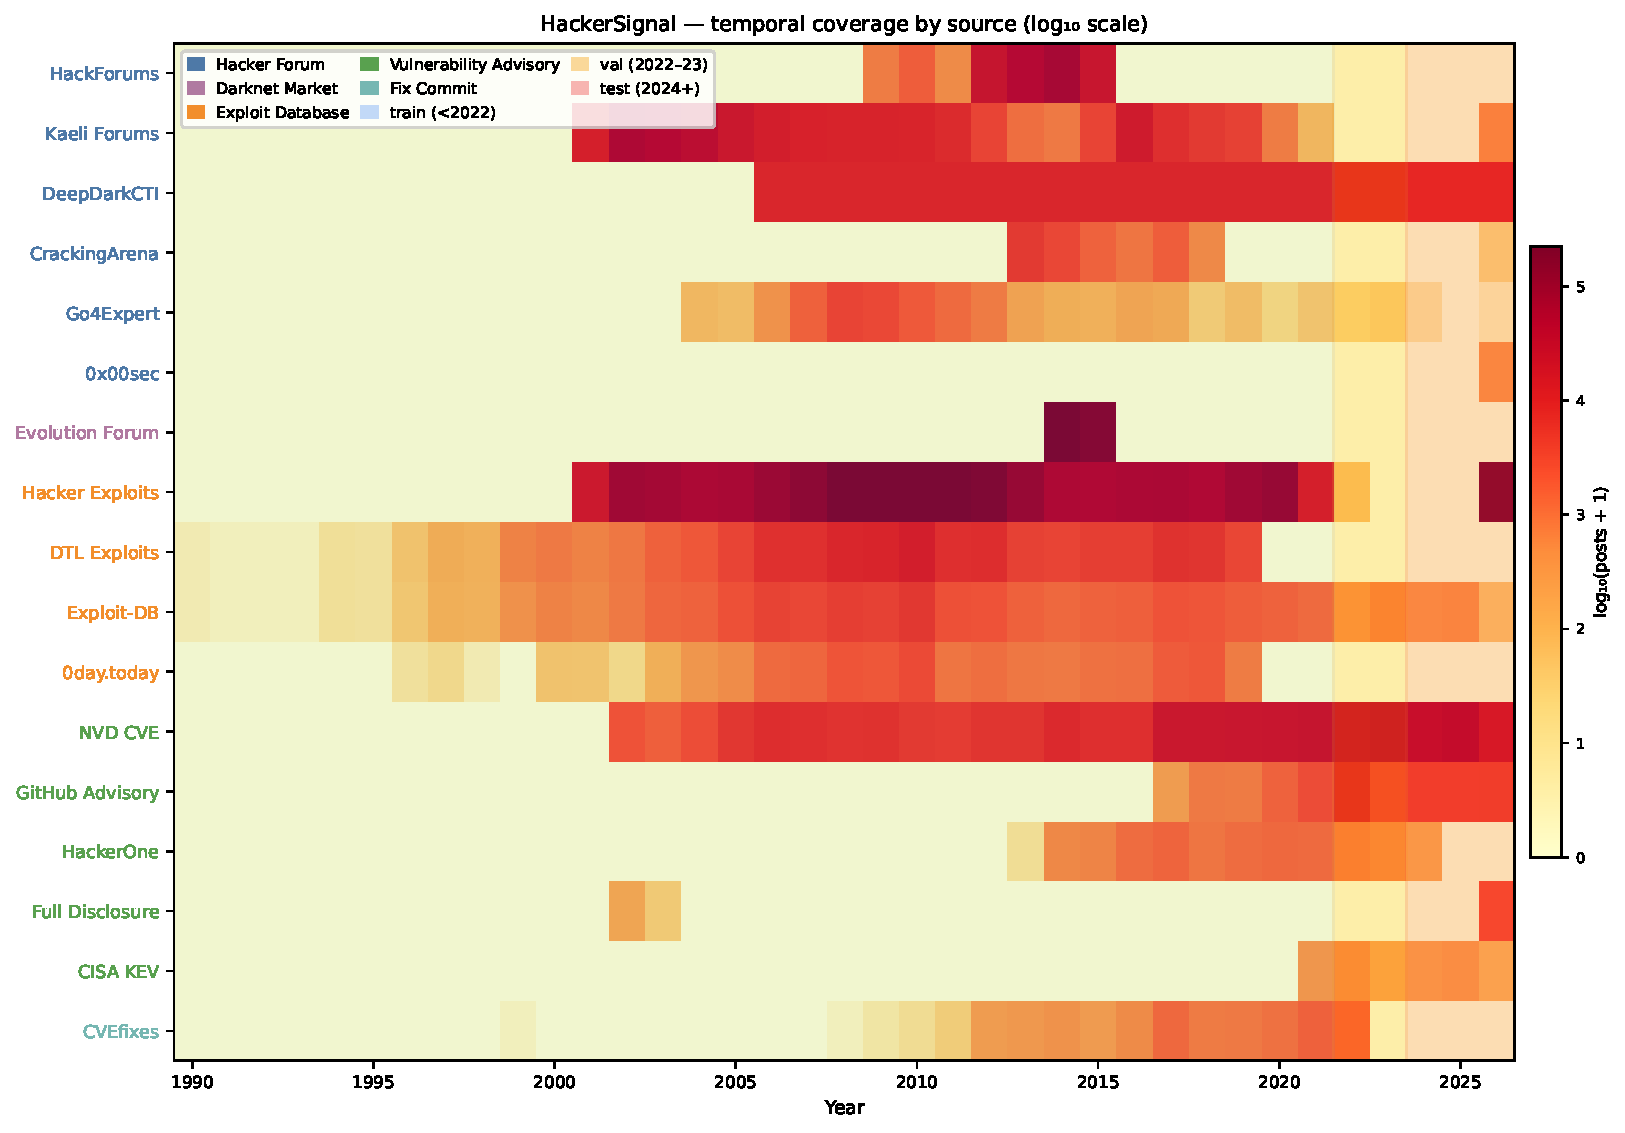
\includegraphics[width=\linewidth]{figures/temporal_heatmap.pdf}
\caption{Temporal coverage by source layer (log$_{10}$ scale). Colored bars indicate benchmark split boundaries: train ($<$2022), val (2022--23), test (2024+).}
\label{fig:temporal-heatmap}
\end{figure}

Several high-volume historical sources (HackForums, Gayanku, Evolution, and the AntiOnline/Go4Expert forums) end in 2015-2017, while newer sources (DeepDarkCTI communities, 0x00sec, HackerSploit, ParrotSec, NVD, GitHub Advisory, and CISA KEV) extend into 2026 (Figure~\ref{fig:temporal-heatmap}). In addition, the corpus is predominantly English. Multilingual content (Russian, Turkish, Persian, Arabic, Chinese) appears in DeepDarkCTI and several dark-market sources. Short rows ($<$8 tokens, 21.1\%) include replies and marketplace acknowledgments. These should be filtered for classification and retrieval tasks, but are useful for other analyses of community interactions.

Past research indicates that hacker community platforms vary in content, such as exploits and tools. To measure lexical similarity among 46 forums, we compute pairwise Jaccard coefficients using a 5\% token sample and perform hierarchical clustering (Figure~ref{fig:domain-overlap}). The heatmap and network show a dense cluster of English-language security forums (hackforums, zerosec, cipher, wilderssecurity, go4expert, cipherspace) with shared technical vocabulary. Dark Web marketplaces (Gayanku, Evolution) form a second cluster connected by transactional terms. Non-English forums (antichat, persiantools) and niche groups (parrotsec, zeroday~today) are peripheral with low overlap ($J < 0.06$), showing language and domain create vocabulary boundaries. Node sizes reflect contribution on a $"log_{10}$ scale, highlighting antichat, gayanku, and wwhclub's prominence in document count despite lexical isolation. This heterogeneity supports our evaluation, as models must generalize across diverse vocabularies.

\begin{figure}[t]
\centering
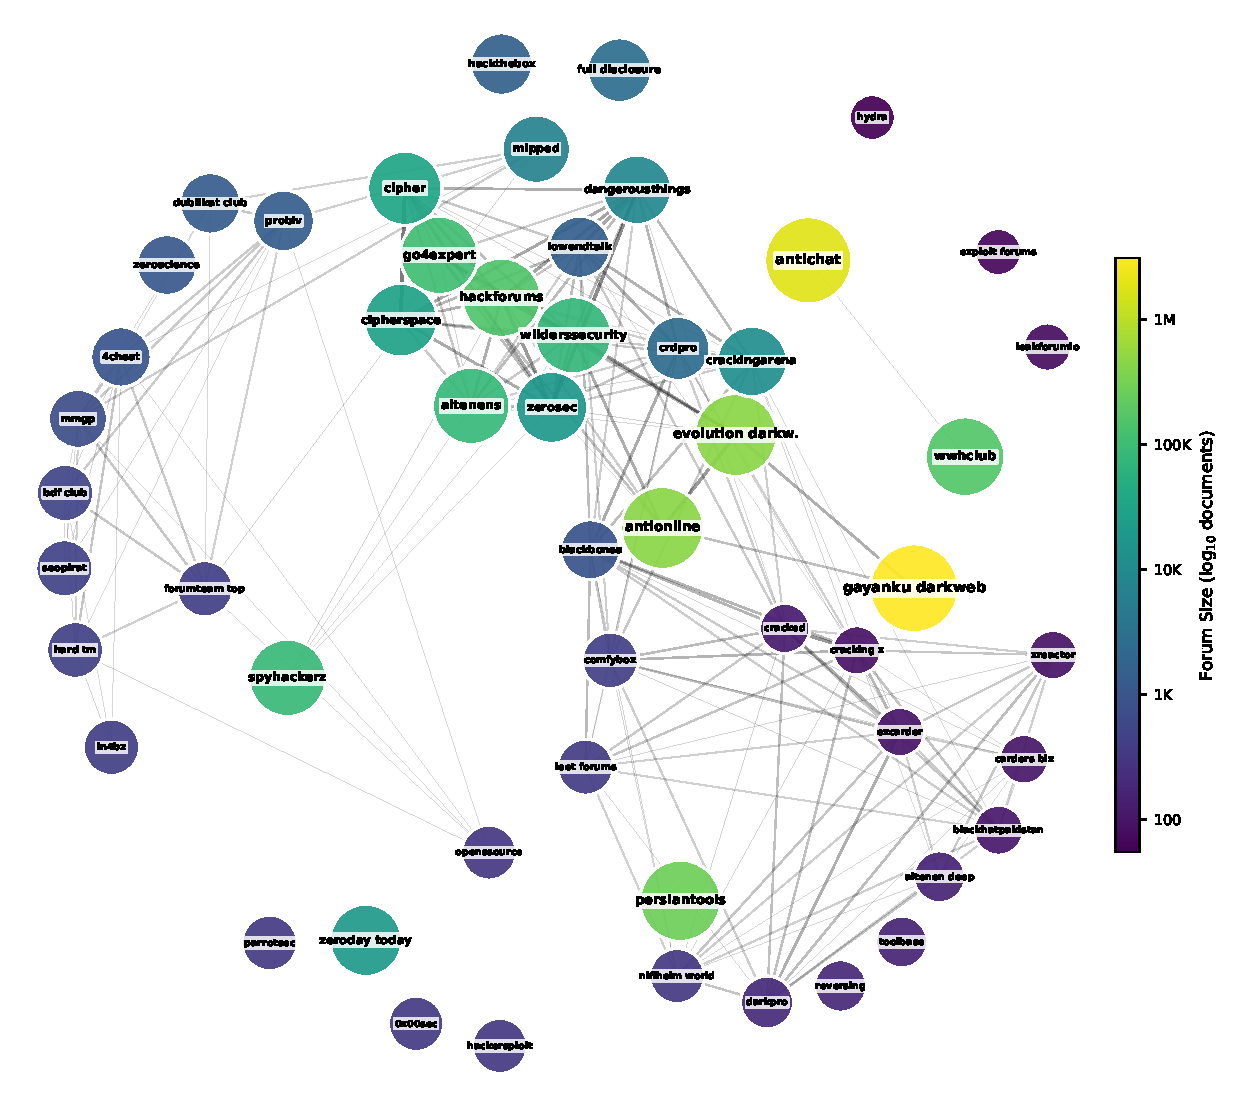
\includegraphics[width=0.8\linewidth]{figures/domain_overlap.pdf}
\caption{Pairwise vocabulary overlap across 46 hacker community forums (5\% deterministic token sample, hierarchically clustered).}
\label{fig:domain-overlap}
\end{figure}

\section{Benchmark Tasks and Results}
\label{sec:tasks}

HackerSignal provides a unique longitidunal, multi-lingual, and multi-sourced CTI dataset that can enable novel research opportunities examining temporal phenomena, generalization, and more. We illustrate three sample CTI tasks with increasing levels methodological complexity that HackerSignal enables in (Figure~\ref{fig:pipeline}, right; Table~\ref{tab:task-summary}). Each probes a different facet of temporal out-of-distribution generalization. All tasks use temporal splits, ensuring that test data postdate training. Following~\citet{thakur2021beir}, we evaluate each task with a heterogeneous baseline ladder spanning lexical, dense, and hybrid methods.

\begin{table}[t]
\centering
\small
\caption{Benchmark task summary. Tasks~1 and~3 use temporal splits (train $<$2022, test 2024+) over the full 340K NVD corpus; Task~2 uses an earlier split (train $<$2020, test $\geq$2023).}
\label{tab:task-summary}
\begin{tabular}{llrrrr}
\toprule
\textbf{Task} & \textbf{Type} & \textbf{Train} & \textbf{Val} & \textbf{Test} & \textbf{Corpus / Total} \\
\midrule
1. CVE-R & Retrieval & 56,692 & 2,584 & 1,990 & 340,536 \\
2. ETC & 8-class classif. & 64,413 & 4,735 & 1,735 & 70,883 \\
3. TG & CVE-disjoint Retr. & 56,833 & 2,535 & 1,898 & 340,536$^\dagger$ \\
\bottomrule
\multicolumn{6}{l}{\footnotesize $^\dagger$Same corpus; zero CVE overlap between train/val/test gold sets.}
\end{tabular}
\end{table}

All benchmark labels are derived from platform-provided and standardized metadata rather than manual annotation (helping reduce third-party biases). Following~\citet{zhang2021wrench}, we explicitly report weak-label sources and aggregation rules, as minor protocol changes can alter benchmark results and conclusions. For retrieval tasks (Tasks~1 and~3), a query's gold CVE is the metadata-linked entry from its source. This may be incomplete or linked to a related rather than maximally specific CVE. For exploit type classification (Task~2), labels are derived from structured metadata fields (ExploitDB exploit type and description, exploit type, HackerOne vulnerability type prefix) and mapped to a unified 8-class taxonomy via deterministic rules. We provide a 240-row stratified manual audit packet in \texttt{data/audits/} for transparency.

\subsection{Task 1: CVE Linkage Retrieval (CVE-R)}
\label{sec:task1}

Let $\mathcal{Q}$ be a set of exploit/advisory evidence texts and $\mathcal{C} = \{c_1, \ldots, c_N\}$ the NVD corpus of $N{=}340{,}536$ CVE descriptions. For each query $q \in \mathcal{Q}$, the task is to retrieve the correct CVE entry $c^* \in \mathcal{C}$ such that the source metadata links $q$ to $c^*$. This is cross-source temporal out-of-domain entity grounding, akin to knowledge-intensive entity linking~\citep{petroni2021kilt}, except the target knowledge base is the CVE ecosystem. Queries come from exploit archives, advisories, fix commits, and bug-bounty reports, while the target space is a single canonical CVE registry. We retain query sources with low or medium CVE-linkage audit risk (CISA~KEV, CVEfixes, HackerOne) and require $\geq$8 query tokens. Labels are metadata-derived linkages, not manually adjudicated ground truth. 

\begin{wraptable}{r}{0.52\textwidth}
\vspace{-4pt}
\centering
\small
\setlength{\tabcolsep}{3pt}
\caption{Task 1 (CVE-R) test results (1,990 queries, 340K corpus).}
\label{tab:task1-results}
\begin{tabular}{lcccc}
\toprule
\textbf{Model} & \textbf{R@1} & \textbf{R@5} & \textbf{R@10} & \textbf{MRR} \\
\midrule
BM25 & 0.445 & 0.640 & 0.707 & 0.528 \\
MiniLM-L6-v2 & 0.431 & 0.656 & 0.727 & 0.530 \\
mpnet-base-v2 & 0.460 & 0.640 & 0.718 & 0.540 \\
BGE-base-v1.5 & 0.429 & 0.666 & 0.742 & 0.534 \\
E5-base-v2 & \textbf{0.493} & \textbf{0.707} & \textbf{0.769} & \textbf{0.587} \\
\midrule
Hybrid BM25+mpnet & 0.486 & 0.675 & 0.736 & 0.567 \\
\bottomrule
\end{tabular}
\vspace{-4pt}
\end{wraptable}

We choose baselines across three dense retrieval paradigms. BM25 is an unsupervised lexical baseline, serving as an exact-match ceiling. For dense bi-encoders, we selected four models differing in pre-training and architecture: (1) MiniLM-L6-v2 (speed-optimized, distilled 6-layer), (2) all-mpnet-base-v2 (mean-pooled MPNet with contrastive training on 1B+ pairs), (3) BGE-base-v1.5 (instruction-tuned bi-encoder from BAAI for zero-shot transfer), and (4) E5-base-v2 (weakly-supervised contrastive model with task-specific prompts). These span distilled vs. full-size and supervised vs. weakly supervised training, helping assess the impact of pre-training on CVE retrieval. Hybrid BM25+mpnet combines lexical and dense scores via reciprocal rank fusion ($ k=60$), testing their complementarity. We measure Recall@$k$ ($ k= {10}$) and MRR, with results in Table~\ref{tab:task1-results}.

The standard bi-encoders (MiniLM, mpnet, BGE) cluster tightly(MRR 0.530-0.540), comparable to BM25. E5-base-v2 substantially outperforms all other models, including the hybrid (MRR~0.587 vs 0.567), likely due to its asymmetric query/passage prefix design, which better separates the retrieval roles. The hybrid combination (normalized BM25 + dense cosine, $\alpha{=}0.7$) reranks BM25 top-100 candidates and outperforms symmetric bi-encoders but not the prefix-trained E5.

\subsection{Task 2: Exploit Type Classification (ETC)}
\label{sec:task2}

Given an exploit text $x$, predict its vulnerability type $y \in \mathcal{Y}$ where $|\mathcal{Y}| = 8$ classes: \emph{injection} (SQLi, command/code injection, XXE), \emph{XSS} (reflected, stored, DOM), \emph{memory corruption} (buffer/heap overflow, use-after-free, format string), \emph{denial of service}, \emph{file inclusion} (LFI/RFI, path traversal, arbitrary file operations), \emph{authentication \& access control} (privilege escalation, auth bypass, CSRF, IDOR), \emph{remote code execution} (RCE, deserialization), and \emph{information disclosure} (SSRF, open redirect, data exposure). This taxonomy aligns with CWE top-level categories and prior exploit classification work~\citep{ampel2020dtl,ampel2024misq}. Labels are derived from structured metadata: ExploitDB exploit descriptions and tags, 0day.today exploit type fields, and HackerOne vulnerability type prefixes. The dataset comprises 70,883 labeled exploit texts from these three source families.

We use a temporal out-of-distribution split (train $<$2020, val 2020-2022, test $\geq$2023) so that models must generalize to vulnerabilities and exploits that postdate training. We evaluate a model ladder spanning bag-of-words classifiers (Decision Tree, TF-IDF+LR, linear SVM), recurrent neural networks (RNN, GRU, LSTM, BiLSTM), and a domain-specific transformer (SecBERT~\citep{secbert2022}). We report macro-F1 and per-class F1 for the three hardest classes in Table~\ref{tab:task2-results}.

\begin{table}[t]
\centering
\small
\setlength{\tabcolsep}{4pt}
\caption{Task 2 (ETC) test results on 1,735 temporally held-out samples. Macro-F1 and per-class F1 for the three hardest classes. BoW = bag-of-words features; Neural = learned representations.}
\label{tab:task2-results}
\begin{tabular}{llcccc}
\toprule
& \textbf{Model} & \textbf{Macro-F1} & \textbf{info\_disc.} & \textbf{mem\_corr.} & \textbf{auth.} \\
\midrule
\multirow{3}{*}{\rotatebox[origin=c]{90}{\footnotesize BoW}}
& Decision Tree     & .708 & .46 & .65 & .60 \\
& TF-IDF + LR       & .772 & .66 & .69 & .79 \\
& SVM (Linear)      & .799 & .70 & .68 & .82 \\
\midrule
\multirow{5}{*}{\rotatebox[origin=c]{90}{\footnotesize Neural}}
& RNN               & .142 & .12 & .10 & .20 \\
& GRU               & .826 & .69 & .78 & .80 \\
& LSTM              & .826 & .68 & .82 & .80 \\
& BiLSTM            & \textbf{.871} & \textbf{.73} & \textbf{.86} & \textbf{.82} \\
& SecBERT           & .846 & .69 & .79 & .82 \\
\bottomrule
\end{tabular}
\end{table}

The best bag-of-words baseline (SVM) attains macro-F1 of 0.799, while BiLSTM reaches 0.871, a 9\% increase over sequential representations. The vanilla RNN performs poorly (macro-F1=0.142), indicating that long exploit texts require more advanced architectures. GRU and LSTM are similar (0.826), with bidirectional models improving results. SecBERT (0.846) surpasses GRU/LSTM but underperforms BiLSTM, suggesting that domain-specific pre-training offers modest benefits, and that bidirectionality is key. The hard classes (information disclosure, memory corruption, authentication/access) have substantial overlap. For example, disclosure exploits often involve injection (SSRF, XXE), while privilege escalation and authentication share patterns with RCE. Decision Tree drops to macro-F1=0.708, with disclosure at 0.46. Lexical classes such as XSS and injection are easier (F1 > 0.82), indicating that exploit signals are partly lexical. Temporal splits make it harder as exploit names and vulnerability patterns evolve, preventing models from memorizing era-specific features.

\subsection{Task 3: Temporal Generalization (TG)}
\label{sec:task3}

Identical retrieval formulation to Task~1, but with a strict CVE-disjointness constraint: $C_{\text{train}} \cap C_{\text{test}} = \emptyset$, where $C_s = \{c^*_i : q_i \in \text{split}~s\}$ is the set of gold CVE targets in split $s$. Splits are defined by CVE publication year rather than query timestamp: train uses CVEs published before 2022, validation uses 2022--2023, and test uses 2024+. This ensures that models cannot memorize vulnerability descriptions seen during training and must generalize to wholly unseen vulnerabilities. We use the same metrics and models as Task~1 and show the results of Task~3 in Table~\ref{tab:task3-results}.

\begin{wraptable}{r}{0.52\textwidth}
\vspace{-4pt}
\centering
\small
\setlength{\tabcolsep}{3pt}
\caption{Task 3 (TG) results (1,898 test queries) under strict CVE disjointness
($C_{\text{train}} \cap C_{\text{test}} = \emptyset$).}
\label{tab:task3-results}
\begin{tabular}{lcccc}
\toprule
\textbf{Model} & \textbf{R@1} & \textbf{R@5} & \textbf{R@10} & \textbf{MRR} \\
\midrule
BM25 & 0.443 & 0.654 & 0.715 & 0.533 \\
MiniLM-L6-v2 & 0.453 & 0.669 & 0.728 & 0.546 \\
mpnet-base-v2 & 0.461 & 0.657 & 0.725 & 0.544 \\
BGE-base-v1.5 & 0.438 & 0.677 & 0.753 & 0.546 \\
E5-base-v2 & \textbf{0.509} & \textbf{0.725} & \textbf{0.779} & \textbf{0.602} \\
\midrule
Hybrid BM25+mpnet & 0.491 & 0.690 & 0.743 & 0.577 \\
\bottomrule
\end{tabular}
\vspace{-4pt}
\end{wraptable}

Under CVE-disjoint evaluation, E5-base (MRR~0.602) exceeds both the hybrid and all symmetric encoders. Models generally maintain or improve performance compared to Task~1, confirming that our temporal split already prevents meaningful memorization. The consistent E5 advantage across both tasks suggests that asymmetric prefix training is particularly effective for cross-source CVE grounding, where queries and targets have different discourse design, as already demonstrated in a rigorous prospective evaluation.

\begin{figure}[t]
\centering
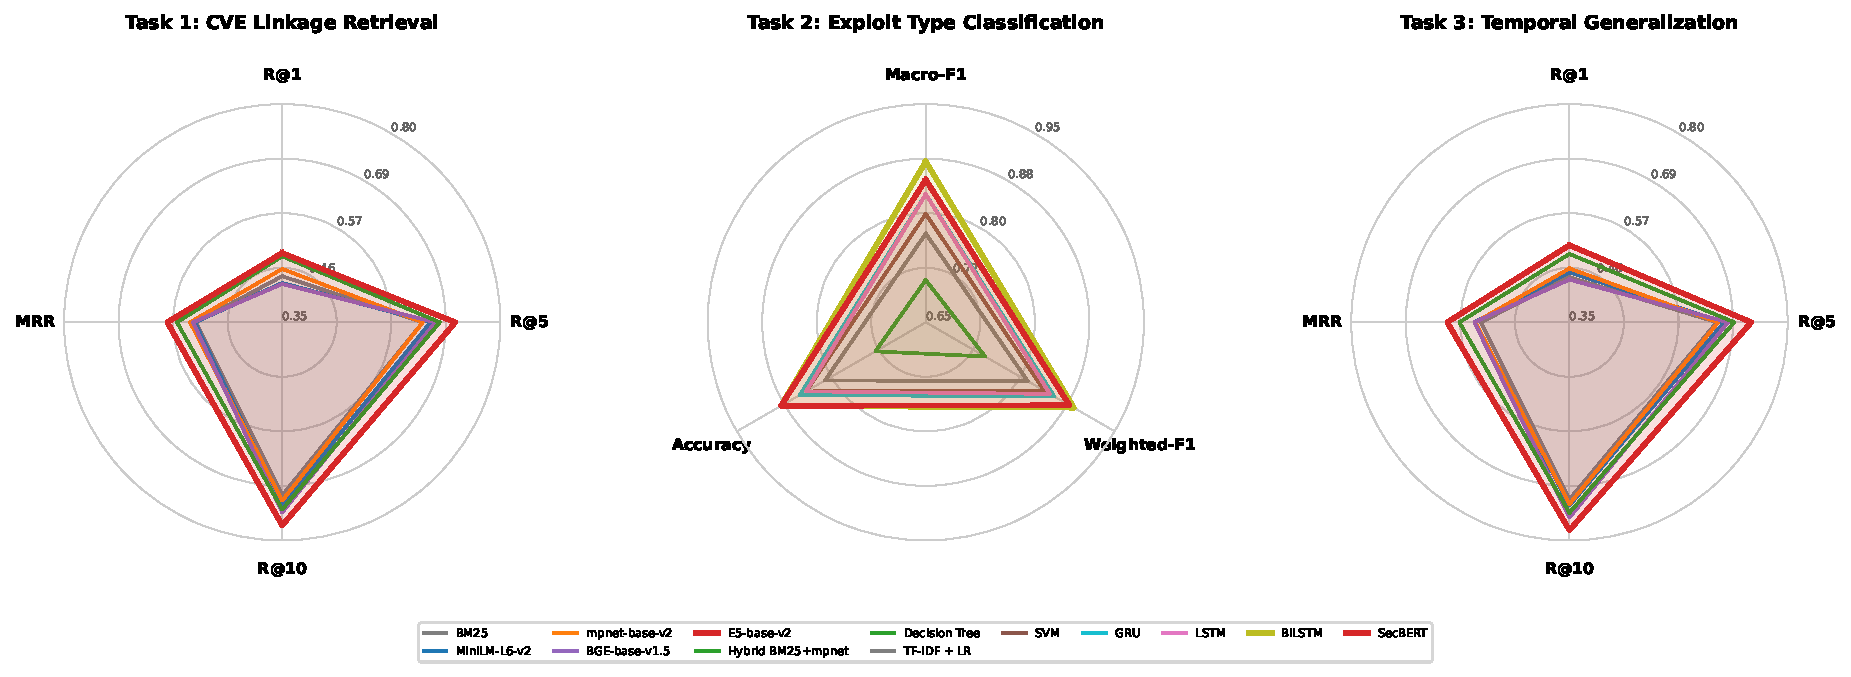
\includegraphics[width=\linewidth]{figures/baseline_results_summary.pdf}
\caption{Radar chart summary of baseline performance across all three tasks.}
\label{fig:baselines-summary}
\end{figure}

\subsection{Audit Artifacts and Error Analysis}

Following~\citet{kapoor2023leakage}, we explicitly audit for temporal and source leakage because benchmark claims are otherwise too easy to inflate. The CVE-disjointness of Task~3 is verified programmatically: $|C_{\text{train}} \cap C_{\text{test}}| = 0$. Full details are in Appendix~\ref{app:audit-reliability}.

Among the Hybrid model's Task~1 errors (queries where the target CVE does not appear in the top-10), we identify three recurring failure patterns: (1)~\emph{Generic exploit descriptions} matching multiple CVEs sharing a common vulnerability class; (2)~\emph{Version-specific queries} referencing product versions absent from the NVD description; and (3)~\emph{Alias mismatches} where queries use informal names (e.g., "Log4Shell") while the NVD entry uses only formal identifiers. E5-base-v2's strong performance (MRR~0.587, exceeding even the hybrid) demonstrates that asymmetric query/passage encoding is well-suited to CVE grounding.

\section{Ethical Considerations}
\label{sec:ethics}

The source mix contains various licenses and terms of service. The public release categorizes sources into redistributable, research-only, metadata/pointer, and excluded. A governance addendum details release modes, contact info, versioning, checksums, and takedown procedures. All sources are accessible without authentication, but privacy risks remain. We pseudonymize author IDs via SHA-256, preserve provenance, and support takedown requests, downgrading ambiguous sources accordingly. HackerSignal highlights vulnerabilities for defensive research only, prohibiting fine-tuning automated exploit models, de-anonymizing forum users, and automated incident response without human review. The governance addendum enforces these rules, including release modes and version management. Researchers should consult IRBs when analyzing individuals. The dataset, available on HuggingFace, is for academic and defensive use only, not operational threat feeds. Outputs should not be trusted as the current CTI without validation. The repository includes metadata, a dataset card, and a link to the governance addendum.

\section{Conclusion}
\label{sec:discussion}

HackerSignal links 7.45M documents from 64 sources across the CVE lifecycle with temporal splits, CVE-disjoint evaluation, and provenance-aware governance. Our three-task benchmark and model ladder (BM25 through E5 retrieval at MRR~0.60, BiLSTM at macro-F1~0.87 for 8-class exploit type classification) establishes baselines for cross-source CVE grounding, exploit type classification, and prospective generalization to unseen vulnerabilities.

Several limitations bound the current release. First, CVE linkages are metadata-derived (source URLs, CVE regex extraction) rather than expert-adjudicated, introducing noise proportional to source quality. We mitigate this via per-source audit risk scores, but cannot guarantee zero false linkages. Second, although some hacker forums contain non-English posts, we do not evaluate cross-lingual retrieval or multilingual baselines. Prior work suggests non-English forums require dedicated approaches~\citep{ebrahimi2020crosslingual}. Third, we do not evaluate large language model rerankers (e.g., GPT-4, Claude) or retrieval-augmented generation pipelines, which may score higher but at orders-of-magnitude higher compute cost.

Beyond the three tasks benchmarked here, the 6.97M-row hacker community subcorpus opens research directions in exploit code summarization and completion, hacker content extraction and labeling, topic modeling (e.g., LDA over forum-specific vocabularies), community interaction network analysis, cross-lingual CTI transfer across the corpus's multilingual forums, and temporal trend detection in exploit discourse. HackerSignal's code, data, splits, and Croissant metadata are publicly released to support these extensions at \href{https://huggingface.co/datasets/DatasetSubmission/HackerSignal}{\texttt{hf.co/datasets/DatasetSubmission/HackerSignal}} (data) and \href{https://anonymous.4open.science/r/hackersignal-8A2F/}{\texttt{anonymous.4open.science/r/hackersignal-8A2F}} (code).

\begin{thebibliography}{99}
\small

\bibitem[Akhtar et~al.(2024)]{croissant2024}
Akhtar, M., et al. (2024). Croissant: A Metadata Format
for ML-Ready Datasets. \textit{NeurIPS 2024 D\&B Track}.

\bibitem[Ampel et~al.(2020)]{ampel2020dtl}
Ampel, B., Samtani, S., Zhu, H., Ullman, S., \& Chen, H. (2020).
Labeling Hacker Exploits for Proactive Cyber Threat Intelligence: A Deep
Transfer Learning Approach. \textit{IEEE Intelligence and Security
Informatics (ISI)}. \url{https://doi.org/10.1109/ISI49825.2020.9280548}.

\bibitem[Ampel et~al.(2024)]{ampel2024misq}
Ampel, B., Samtani, S., Zhu, H., \& Chen, H. (2024).
Creating Proactive Cyber Threat Intelligence with Hacker Exploit Labels:
A Deep Transfer Learning Approach. \textit{MIS Quarterly}, 48(1), 137--166.

\bibitem[Robertson and Jones(1994)]{bm25robertson1994}
Robertson, S., \& Jones, K.\ S. (1994).
Simple, proven approaches to text retrieval.
\textit{Technical report}, University of Cambridge.

\bibitem[Thakur et~al.(2021)]{thakur2021beir}
Thakur, N., Reimers, N., R{\"u}ckl{\'e}, A., Srivastava, A., \&
Gurevych, I. (2021). BEIR: A Heterogeneous Benchmark for Zero-shot
Evaluation of Information Retrieval Models. \textit{NeurIPS 2021 D\&B
Track}. arXiv:2104.08663.

\bibitem[CISA(2021--2026)]{cisakev}
CISA. (2021--2026). Known Exploited Vulnerabilities Catalog.
\url{https://www.cisa.gov/known-exploited-vulnerabilities-catalog}.

\bibitem[Pastrana et~al.(2018)]{crimebb2018}
Pastrana, S., Thomas, D.\ R., Hutchings, A., \&
Caines, A. (2018). CrimeBB: Enabling Cybercrime Research on Underground
Forums at Scale. \textit{WWW 2018}.

\bibitem[Deliu et~al.(2017)]{deliu2017cti}
Deliu, I., Leichter, C., \& Franke, K. (2017).
Extracting Cyber Threat Intelligence from Hacker Forums: Support Vector
Machines versus Convolutional Neural Networks.
\textit{IEEE International Conference on Big Data}.
\url{https://doi.org/10.1109/BigData.2017.8258359}.

\bibitem[Bhandari et~al.(2021)]{cvefixes2021}
Bhandari, G., Naseer, A., \& Moonen, L. (2021).
CVEfixes: Automated Collection of Vulnerabilities and Their Fixes from
Open-Source Software. \textit{PROMISE 2021}.

\bibitem[Ranade et~al.(2021)]{cysecbert2021}
Ranade, P., Piplai, A., Mittal, S., Joshi, A., \&
Finin, T. (2021). CyBERT: BERT for cybersecurity natural language
processing. \textit{Computing}.

\bibitem[Devlin et~al.(2019)]{devlin2019bert}
Devlin, J., Chang, M.-W., Lee, K., \& Toutanova, K.
(2019). BERT: Pre-training of Deep Bidirectional Transformers for
Language Understanding. \textit{NAACL 2019}.

\bibitem[Ebrahimi et~al.(2020)]{ebrahimi2020crosslingual}
Ebrahimi, M., Samtani, S., Chai, Y., \& Chen, H. (2020).
Detecting Cyber Threats in Non-English Hacker Forums: An Adversarial
Cross-Lingual Knowledge Transfer Approach.
\textit{IEEE Security and Privacy Workshops}, 20--26.
\url{https://doi.org/10.1109/SPW50608.2020.00021}.

\bibitem[Offensive Security(2003--2026)]{exploitdb}
Offensive Security. (2003--2026). Exploit Database.
\url{https://www.exploit-db.com/}. Licensed CC BY-SA 4.0.

\bibitem[Gayanku(2020)]{gayanku2020}
Gayanku. (2020). Hacker Forum Posts Dataset.
\textit{Kaggle}. \url{https://www.kaggle.com/gayanku}.

\bibitem[Gebru et~al.(2021)]{gebru2021datasheet}
Gebru, T., et al. (2021). Datasheets for Datasets.
\textit{Communications of the ACM}, 64(12), 86--92.

\bibitem[Cohen(1960)]{cohen1960kappa}
Cohen, J. (1960). A coefficient of agreement for nominal scales.
\textit{Educational and Psychological Measurement}, 20(1), 37--46.
\url{https://doi.org/10.1177/001316446002000104}.

\bibitem[GitHub(2017--2026)]{githubadvisory}
GitHub. (2017--2026). GitHub Advisory Database.
\url{https://github.com/advisories}. Licensed CC BY 4.0.

\bibitem[Grisham et~al.(2017)]{grisham2017mobile}
Grisham, J., Samtani, S., Patton, M., \& Chen, H. (2017).
Identifying Mobile Malware and Key Threat Actors in Online Hacker Forums
for Proactive Cyber Threat Intelligence.
\textit{IEEE Intelligence and Security Informatics (ISI)}.

\bibitem[Otto et~al.(2021)]{otto2021isi}
Otto, K., Ampel, B., Samtani, S., Zhu, H., \& Chen, H. (2021).
Exploring the Evolution of Exploit-Sharing Hackers: An Unsupervised
Graph Embedding Approach. \textit{IEEE Intelligence and Security
Informatics (ISI)}. \url{https://doi.org/10.1109/ISI53945.2021.9624846}.

\bibitem[NIST(2002--2026)]{nvd}
NIST. (2002--2026). National Vulnerability Database.
\url{https://nvd.nist.gov/}. Public domain.

\bibitem[Petroni et~al.(2021)]{petroni2021kilt}
Petroni, F., Piktus, A., Fan, A., Lewis, P., Yazdani, M., et al.
(2021). KILT: A Benchmark for Knowledge Intensive Language Tasks.
\textit{NAACL 2021}. \url{https://doi.org/10.18653/v1/2021.naacl-main.200}.

\bibitem[Nunes et~al.(2016)]{nunes2016darknet}
Nunes, E., Diab, A., Gunn, A., Marin, E., Mishra, V.,
Paliath, V., Robertson, J., Shakarian, J., Thart, A., \&
Shakarian, P. (2016). Darknet and Deepnet Mining for Proactive
Cybersecurity Threat Intelligence. \textit{IEEE Intelligence and
Security Informatics (ISI)}.

\bibitem[Jackaduma(2022)]{secbert2022}
Jackaduma. (2022). SecBERT: A Pre-trained Language Model
for Cybersecurity. \url{https://huggingface.co/jackaduma/SecBERT}.

\bibitem[Krippendorff(2008)]{krippendorff2008alpha}
Krippendorff, K. (2008). Systematic and random disagreement and the
reliability of nominal data. \textit{Communication Methods and Measures},
2(4), 323--338. \url{https://doi.org/10.1080/19312450802467134}.

\bibitem[Gwet(2014)]{gwet2014handbook}
Gwet, K.\ L. (2014). \textit{Handbook of Inter-Rater Reliability}.
Advanced Analytics.

\bibitem[Kapoor and Narayanan(2023)]{kapoor2023leakage}
Kapoor, S., \& Narayanan, A. (2023). Leakage and the Reproducibility
Crisis in Machine-Learning-Based Science. \textit{Patterns}, 4(9),
100804. \url{https://doi.org/10.1016/j.patter.2023.100804}.

\bibitem[Koh et~al.(2021)]{koh2021wilds}
Koh, P.\ W., Sagawa, S., Marklund, H., Xie, S.\ M., Zhang, M.,
et al. (2021). WILDS: A Benchmark of in-the-Wild Distribution Shifts.
\textit{ICML 2021}, PMLR 139.

\bibitem[Han et~al.(2017)]{severitypred2017}
Han, D., et al. (2017). Learning to Predict Severity
of Software Vulnerability Using Only Vulnerability Description.
\textit{ICSME 2017}.

\bibitem[Reimers and Gurevych(2019)]{sbert2019}
Reimers, N., \& Gurevych, I. (2019). Sentence-BERT:
Sentence Embeddings using Siamese BERT-Networks. \textit{EMNLP 2019}.

\bibitem[Samtani et~al.(2015)]{samtani2015assets}
Samtani, S., Chinn, R., \& Chen, H. (2015).
Exploring Hacker Assets in Underground Forums.
\textit{IEEE Intelligence and Security Informatics (ISI)}, 31--36.
\url{https://doi.org/10.1109/ISI.2015.7165935}.

\bibitem[Samtani et~al.(2017)]{samtani2017jmis}
Samtani, S., Chinn, R., Chen, H., \& Nunamaker, J.\ F. (2017).
Exploring Emerging Hacker Assets and Key Hackers for Proactive Cyber
Threat Intelligence. \textit{Journal of Management Information Systems},
34(4), 1023--1053. \url{https://doi.org/10.1080/07421222.2017.1394049}.

\bibitem[Samtani et~al.(2020)]{samtani2020dgef}
Samtani, S., Zhu, H., \& Chen, H. (2020).
Proactively Identifying Emerging Hacker Threats from the Dark Web: A
Diachronic Graph Embedding Framework. \textit{ACM Transactions on Privacy
and Security}, 23(4), Article 21. \url{https://doi.org/10.1145/3409289}.

\bibitem[Samtani et~al.(2021)]{samtani2021hap}
Samtani, S., Li, W., Benjamin, V., \& Chen, H. (2021).
Informing Cyber Threat Intelligence through Dark Web Situational
Awareness: The AZSecure Hacker Assets Portal. \textit{Digital Threats:
Research and Practice}, 2(4), Article 27.
\url{https://doi.org/10.1145/3450972}.

\bibitem[Samtani et~al.(2022)]{samtani2022eva}
Samtani, S., Chai, Y., \& Chen, H. (2022).
Linking Exploits from the Dark Web to Known Vulnerabilities for Proactive
Cyber Threat Intelligence: An Attention-Based Deep Structured Semantic
Model. \textit{MIS Quarterly}, 46(2), 911--946.

\bibitem[Zhang et~al.(2021)]{zhang2021wrench}
Zhang, J., Yu, Y., Li, Y., Wang, Y., Yang, Y., Yang, M., \&
Ratner, A. (2021). WRENCH: A Comprehensive Benchmark for Weak
Supervision. \textit{NeurIPS 2021 D\&B Track}. arXiv:2109.11377.

\bibitem[Rahman et~al.(2023)]{rahman2023cti}
Rahman, M.\ R., Mahdavi-Hezaveh, R., \& Williams, L. (2023).
What Are the Attackers Doing Now? Automating Cyberthreat Intelligence
Extraction from Text on Pace with the Changing Threat Landscape: A Survey.
\textit{ACM Computing Surveys}, 55(12), Article~254.
\url{https://doi.org/10.1145/3571726}.

\bibitem[Hughes et~al.(2024)]{hughes2024cybercrime}
Hughes, J., Pastrana, S., Hutchings, A., Afroz, S., Samtani, S.,
Li, W., \& Marin, E.\ S. (2024).
The Art of Cybercrime Community Research.
\textit{ACM Computing Surveys}, 56(6), Article~155.
\url{https://doi.org/10.1145/3639362}.

\end{thebibliography}

\appendix

\section{Source Collection Details}
\label{app:collection}

The full source-by-source matrix and takedown/correction process are in \texttt{docs/release\_governance.md}. Collection scripts are available at \href{https://anonymous.4open.science/r/hackersignal-8A2F/}{\texttt{anonymous.4open.science/r/hackersignal-8A2F}} under \texttt{src/etg/collectors/}. The public JSONL release is built from the full research build by enforcing \texttt{release\_mode}: rows from \texttt{metadata\_or\_pointer\_only} sources retain provenance, timestamps, source/thread identifiers, CVE references, text hashes, and text lengths, but \texttt{text} and \texttt{text\_raw} are withheld. Table~\ref{tab:collection-details} provides per-source collection method, access mechanism, license posture, and default release mode.

\begin{table}[t]
\centering
\small
\caption{Per-source collection details.}
\label{tab:collection-details}
\begin{tabular}{lllll}
\toprule
\textbf{Source} & \textbf{Method} & \textbf{Access} & \textbf{License} & \textbf{Release mode} \\
\midrule
NVD             & REST API        & Public & Public domain & Text \\
CISA KEV        & JSON feed       & Public & Public domain & Text \\
GitHub Advisory & GraphQL API     & Public & CC BY 4.0 & Text \\
ExploitDB       & CSV download    & Public & CC BY-SA 4.0 & Text \\
HackerOne       & HuggingFace Hub & Public & Source dataset terms & Research text \\
CVEfixes        & Zenodo SQLite   & Public & CC BY 4.0 & Text \\
Kaggle forums   & Kaggle          & Public & Dataset-specific & Research/pointer \\
DeepDarkCTI     & GitHub          & Public & Repository terms & Research text \\
0x00sec/HTB/etc.& Discourse API   & Public & Site terms & Pointer \\
Other web archives & Web scraping & Public & Mixed terms & Pointer \\
\bottomrule
\end{tabular}
\end{table}

\section{Audit and Reliability}
\label{app:audit-reliability}

We follow the audit framework of~\citet{kapoor2023leakage} and perform three complementary integrity checks. First, for each task, we draw a 80-row stratified random sample (240 rows total, balanced across splits) and manually verify (i)~correct CVE assignment, (ii)~temporal split adherence, and (iii)~absence of trivial textual overlap between query and target. No errors were found. Second, we search for exact and near-duplicate text spans between train and test partitions using MinHash (Jaccard threshold $\geq$0.8, 128 permutations). After deduplication during corpus construction, zero train-test pairs exceed the threshold for any task. Finally, we verify that no CVE identifier appears in both the train and test for any task. For Task~3 (temporal generalization), CVE-disjointness is enforced by construction: $|C_{\text{train}} \cap C_{\text{test}}| = 0$, supported programmatically at build time.

\section{Model Ladder Details}
\label{app:model-ladder}

The full model ladder evaluates six retrieval approaches (Tasks~1 and~3) and eight classification approaches (Task~2). Each model represents a rung on the complexity ladder from lexical to neural to hybrid methods. BM25 uses no learned parameters; bi-encoders (MiniLM, mpnet, BGE, E5) use pre-trained sentence embeddings without task-specific fine-tuning; the hybrid combines BM25 top-100 reranking with dense scores ($\alpha{=}0.7$). For Task~2, the ladder spans bag-of-words classifiers (Decision Tree, TF-IDF + LR, linear SVM), recurrent neural networks (RNN, GRU, LSTM, BiLSTM), and a domain-specific transformer (SecBERT).

\section{Baseline Hyperparameter Details}
\label{app:hyperparams}

\paragraph{BM25 (Tasks 1 and 3).} 
Okapi BM25 via \texttt{rank\_bm25} (BM25Okapi). Tokenization: lowercase whitespace split. Full 340,536-record corpus indexed.

\paragraph{Dense bi-encoders (Tasks 1 and 3).}
Four sentence-transformer models evaluated without task-specific fine-tuning: \texttt{all-MiniLM-L6-v2} (22M params, 384-dim), \texttt{all-mpnet-base-v2} (110M, 768-dim), \texttt{BAAI/bge-base-en-v1.5} (110M, 768-dim), and \texttt{intfloat/e5-base-v2} (110M, 768-dim, with ``query:''/``passage:'' prefixes). Batch size 128, max sequence length 512 tokens, $\ell_2$-normalized embeddings, cosine similarity scoring. Corpus encoded in 5K-document chunks on CPU with multi-process pooling.

\paragraph{Hybrid BM25 + dense (Tasks 1 and 3).}
A combination of normalized BM25 scores and dense cosine similarity with $\alpha{=}0.7$ (dense weight). For efficiency, BM25 retrieves top-100 candidates per query; dense scores are computed only for the candidate set. Final ranking uses $\alpha \cdot \text{dense} + (1{-}\alpha) \cdot \text{BM25}$.

\paragraph{Bag-of-words classifiers (Task 2).}
All BoW classifiers use scikit-learn with \texttt{TfidfVectorizer}(max\_features=50{,}000, ngram\_range=(1,2)) as the feature extractor. \texttt{DecisionTreeClassifier}: max\_depth=30, class\_weight=``balanced''. \texttt{LogisticRegression}: C=1.0, max\_iter=1000, class\_weight=``balanced''. \texttt{LinearSVC}: max\_iter=2000, class\_weight=``balanced''.

\paragraph{Neural classifiers (Task 2).}
RNN, GRU, LSTM, and BiLSTM use a word-level vocabulary (min frequency $\geq$3, yielding ${\sim}$19K tokens) with 128-dim embeddings, 128-dim hidden states, max sequence length 300, batch size 128, and Adam optimizer (lr=$10^{-3}$). Class-weighted cross-entropy loss with gradient clipping at 1.0. Trained for 8 epochs with best checkpoint selected by validation macro-F1. SecBERT~\citep{secbert2022} uses \texttt{jackaduma/SecBERT} with max sequence length 256, batch size 16, AdamW (lr=$2{\times}10^{-5}$, weight decay 0.01), linear warmup over 10\% of steps, trained for 3 epochs on a 15K subsample. All neural models use MPS (Apple Silicon) acceleration.

\paragraph{Compute.}
All baselines ran on a single macOS arm64 workstation (Apple M-series, 16\,GB RAM) with Python 3.12 and PyTorch 2.x. No CUDA GPUs were used. BM25 over 340K corpus: ${\sim}$25 min per task (pure Python). Dense encoding of 340K corpus: ${\sim}$20 min (MiniLM) to ${\sim}$90 min (base-sized models) on CPU. RNN/GRU/LSTM/BiLSTM training: ${\sim}$3 min each (8 epochs on MPS). SecBERT fine-tuning: ${\sim}$90 min (3 epochs, 15K samples on MPS). All baseline code is available at \href{https://anonymous.4open.science/r/hackersignal-8A2F/}{\texttt{anonymous.4open.science/r/hackersignal-8A2F}}.

\section{Comparison with Prior CTI Datasets}
\label{app:comparison}

Table~\ref{tab:dataset-comparison} positions HackerSignal against prior cyber threat intelligence datasets. We emphasize four differentiators: (i) governed public release with source-specific access modes; (ii) temporal benchmark splits enabling prospective evaluation; (iii) cross-source CVE linkage connecting hacker discourse to formal vulnerability records; and (iv) scale exceeding prior resources by an order of magnitude.

\begin{table}[t]
\centering
\small
\setlength{\tabcolsep}{3pt}
\caption{Comparison of HackerSignal with prior CTI datasets across key
dimensions. \cmark{} = yes, \xmark{} = no, $\sim$ = partial.}
\label{tab:dataset-comparison}
\resizebox{\linewidth}{!}{%
\begin{tabular}{lccccccc}
\toprule
\textbf{Dataset} & \textbf{Size} & \textbf{Sources} & \textbf{Public} & \textbf{CVE Link} & \textbf{Temp.\ Splits} & \textbf{Governance} & \textbf{Benchmark} \\
\midrule
CrimeBB~\citep{crimebb2018} & 48M posts & 4 forums & \xmark{} & \xmark{} & \xmark{} & \xmark{} & \xmark{} \\
Gayanku~\citep{gayanku2020} & 3.8M posts & 7 markets & \cmark{} & \xmark{} & \xmark{} & \xmark{} & \xmark{} \\
Otto et al.~\citep{otto2021isi} & 259K posts & 3 forums & \cmark{} & \xmark{} & \xmark{} & \xmark{} & \xmark{} \\
ExploitDB~\citep{exploitdb} & 50K+ & 1 archive & \cmark{} & $\sim$ & \xmark{} & \cmark{} & \xmark{} \\
CVEfixes~\citep{cvefixes2021} & 8.3K & commits & \cmark{} & \cmark{} & \xmark{} & \cmark{} & \xmark{} \\
\midrule
\textbf{HackerSignal (ours)} & \textbf{7.45M} & \textbf{64 sources} & \cmark{} & \cmark{} & \cmark{} & \cmark{} & \cmark{} \\
\bottomrule
\end{tabular}
}
\end{table}

\section{Datasheet}
\label{app:datasheet}

A complete datasheet is provided in the supplemental material and in the dataset repository at \texttt{docs/datasheet.md}~\citep{gebru2021datasheet}.

\newpage
\section*{NeurIPS Paper Checklist}

\begin{enumerate}

\item {\bf Claims}
    \item[] Question: Do the main claims made in the abstract and introduction accurately reflect the paper's contributions and scope?
    \item[] Answer: \answerYes{}
    \item[] Justification: The abstract states three concrete contributions (corpus, benchmark tasks, baselines) that are fully realized in Sections~\ref{sec:dataset} and~\ref{sec:tasks}.

\item {\bf Limitations}
    \item[] Question: Does the paper discuss the limitations of the work performed by the authors?
    \item[] Answer: \answerYes{}
\item[] Justification: Section~\ref{sec:dataset} discusses data quality (duplicates, temporal imbalance, label noise) and Section~\ref{sec:discussion} enumerates four explicit limitations: label provenance, English dominance, missing LLM baselines, and compute constraints.

\item {\bf Theory assumptions and proofs}
    \item[] Question: For each theoretical result, does the paper provide the full set of assumptions and a complete proof?
    \item[] Answer: \answerNA{}
    \item[] Justification: This is a dataset paper with no theoretical results.

\item {\bf Experimental result reproducibility}
    \item[] Question: Does the paper fully disclose all information needed to reproduce the main experimental results?
    \item[] Answer: \answerYes{}
    \item[] Justification: All baseline hyperparameters are reported in Appendix~\ref{app:hyperparams}. Code is released at \href{https://anonymous.4open.science/r/hackersignal-8A2F/}{\texttt{anonymous.4open.science/r/hackersignal-8A2F}}. Data is publicly available on HuggingFace Hub.

\item {\bf Open access to data and code}
    \item[] Question: Does the paper provide open access to the data and code?
    \item[] Answer: \answerYes{}
    \item[] Justification: Dataset released on HuggingFace with provenance metadata, Croissant metadata, and a release-governance addendum. Collection and baseline code released at \href{https://anonymous.4open.science/r/hackersignal-8A2F/}{\texttt{anonymous.4open.science/r/hackersignal-8A2F}}. Accessible without personal request to the PI, with pointer-only modes for sources whose terms do not support text mirroring.

\item {\bf Experimental setting/details}
    \item[] Question: Does the paper specify all training and test details necessary to understand the results?
    \item[] Answer: \answerYes{}
    \item[] Justification: Split boundaries, sources, and hyperparameters are specified in Section~\ref{sec:tasks} and Appendix~\ref{app:hyperparams}.

\item {\bf Experiment statistical significance}
    \item[] Question: Does the paper report error bars or statistical significance?
    \item[] Answer: \answerYes{}
    \item[] Justification: BM25 and dense-retrieval baselines are deterministic given the corpus and produce point estimates. BoW classification baselines (Decision Tree, LR, SVM) use fixed random seeds and deterministic feature extraction. Neural classifiers (RNN, GRU, LSTM, BiLSTM, SecBERT) use fixed random seeds but MPS/GPU training introduces minor nondeterminism; we report single-run results, which is standard for dataset baseline papers. The hybrid retrieval reranks a deterministic BM25 top-100 list.

\item {\bf Experiments compute resources}
    \item[] Question: Does the paper provide sufficient information on compute resources?
    \item[] Answer: \answerYes{}
    \item[] Justification: Baselines were run on a single macOS arm64 workstation with Python 3.12 and PyTorch 2.x. Appendix~\ref{app:hyperparams} reports wall-clock times per model and task.

\item {\bf Code of ethics}
    \item[] Question: Does the research conform with the NeurIPS Code of Ethics?
    \item[] Answer: \answerYes{}
    \item[] Justification: Data are public OSINT, but the paper treats public availability as insufficient by itself: authors are pseudonymized, ambiguous sources can be released pointer-only, and dual-use/takedown restrictions are stated in Section~\ref{sec:ethics} and the governance addendum.

\item {\bf Broader impacts}
    \item[] Question: Does the paper discuss both positive and negative societal impacts?
    \item[] Answer: \answerYes{}
    \item[] Justification: Section~\ref{sec:ethics} addresses dual-use risk, pseudonymization, and prohibited uses.

\item {\bf Safeguards}
    \item[] Question: Does the paper describe safeguards for responsible release?
    \item[] Answer: \answerYes{}
    \item[] Justification: Explicit prohibited uses listed in Section~\ref{sec:ethics} and the governance addendum. Author pseudonymization applied at preprocessing time; disputed or terms-ambiguous sources can be downgraded to metadata/pointer-only release.

\item {\bf Licenses for existing assets}
    \item[] Question: Are existing assets properly credited with licenses?
    \item[] Answer: \answerYes{}
    \item[] Justification: Appendix~\ref{app:collection} lists the license for every source. The References section cites all dataset papers.

\item {\bf New assets}
    \item[] Question: Are new assets well documented?
    \item[] Answer: \answerYes{}
    \item[] Justification: A Gebru et al.\ datasheet is provided (Appendix~\ref{app:datasheet} and \texttt{docs/datasheet.md}). Croissant machine-readable metadata is distributed with the HuggingFace repository.

\item {\bf Crowdsourcing and research with human subjects}
    \item[] Question: Does the paper include details for crowdsourcing or research with human subjects?
    \item[] Answer: \answerNA{}
    \item[] Justification: No crowdsourcing was conducted. The release uses public OSINT sources, pseudonymizes authors, supports takedown/correction requests, and instructs researchers making individual-level inferences to seek their own IRB review.

\item {\bf Institutional review board (IRB) approvals}
    \item[] Question: Does the paper describe IRB approvals for research with human subjects?
    \item[] Answer: \answerNA{}
    \item[] Justification: Collection of public OSINT data was not classified as human-subjects research under institutional guidelines; the paper still documents privacy safeguards, responsible-use restrictions, and release-mode controls.

\item {\bf Declaration of LLM usage}
    \item[] Question: Does the paper describe usage of LLMs as an important component of the core methods?
    \item[] Answer: \answerYes{}
    \item[] Justification: LLMs were not used to create benchmark labels. Writing assistance was also used for editing.

\end{enumerate}

\end{document}
